\documentclass{minimal}
\usepackage{graphicx,color}
\usepackage[utf8]{inputenc}
\usepackage[papersize={420.00bp,298.00bp},text={420.00bp,298.00bp}]{geometry}
\begin{document}
\centering
% Title: gl2ps_renderer figure
% Creator: GL2PS 1.4.2, (C) 1999-2020 C. Geuzaine
% For: Octave
% CreationDate: Mon Dec 12 15:32:56 2022
\setlength{\unitlength}{1pt}
\begin{picture}(0,0)
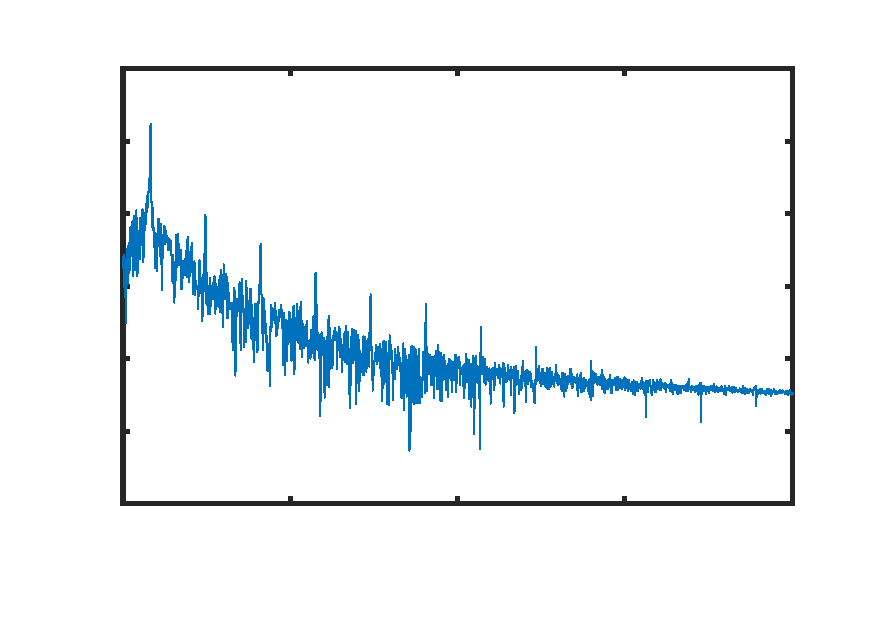
\includegraphics[scale=1]{DoubleFourierTheta1-inc}
\end{picture}%
\begin{picture}(420,298)(0,0)
\fontsize{20}{0}\selectfont\put(59.008,41.3695){\makebox(0,0)[t]{\textcolor[rgb]{0.15,0.15,0.15}{{0}}}}
\fontsize{20}{0}\selectfont\put(139.323,41.3695){\makebox(0,0)[t]{\textcolor[rgb]{0.15,0.15,0.15}{{0.005}}}}
\fontsize{20}{0}\selectfont\put(219.637,41.3695){\makebox(0,0)[t]{\textcolor[rgb]{0.15,0.15,0.15}{{0.01}}}}
\fontsize{20}{0}\selectfont\put(299.952,41.3695){\makebox(0,0)[t]{\textcolor[rgb]{0.15,0.15,0.15}{{0.015}}}}
\fontsize{20}{0}\selectfont\put(380.266,41.3695){\makebox(0,0)[t]{\textcolor[rgb]{0.15,0.15,0.15}{{0.02}}}}
\fontsize{20}{0}\selectfont\put(49,56.3447){\makebox(0,0)[r]{\textcolor[rgb]{0.15,0.15,0.15}{{-5}}}}
\fontsize{20}{0}\selectfont\put(49,91.1206){\makebox(0,0)[r]{\textcolor[rgb]{0.15,0.15,0.15}{{0}}}}
\fontsize{20}{0}\selectfont\put(49,125.896){\makebox(0,0)[r]{\textcolor[rgb]{0.15,0.15,0.15}{{5}}}}
\fontsize{20}{0}\selectfont\put(49,160.672){\makebox(0,0)[r]{\textcolor[rgb]{0.15,0.15,0.15}{{10}}}}
\fontsize{20}{0}\selectfont\put(49,195.448){\makebox(0,0)[r]{\textcolor[rgb]{0.15,0.15,0.15}{{15}}}}
\fontsize{20}{0}\selectfont\put(49,230.224){\makebox(0,0)[r]{\textcolor[rgb]{0.15,0.15,0.15}{{20}}}}
\fontsize{20}{0}\selectfont\put(49,265){\makebox(0,0)[r]{\textcolor[rgb]{0.15,0.15,0.15}{{25}}}}
\fontsize{22}{0}\selectfont\put(219.637,21.3695){\makebox(0,0)[t]{\textcolor[rgb]{0.15,0.15,0.15}{{Frequency}}}}
\fontsize{22}{0}\selectfont\put(22,160.672){\rotatebox{90}{\makebox(0,0)[b]{\textcolor[rgb]{0.15,0.15,0.15}{{log(Power Spectra)}}}}}
\fontsize{22}{0}\selectfont\put(219.637,275){\makebox(0,0)[b]{\textcolor[rgb]{0,0,0}{{Power Spectra of $\theta_1$}}}}
\end{picture}
\end{document}
